\section{Exercise eleven}

Consider now the code:
\begin{verbnobox}[\verbarg]
ADDI S3, S2, 2
ADD S5, S4, S3
SW S5, 4(S3)
SUB S7, S5, S6
LS S6, 4(S7)
\end{verbnobox}
\begin{enumerate}
    \item Find the conflicts. 
    \item Simple Pipelining. 
    \item Reschedule the instructions to reduce the stalls; Draw the pipeline schema showing all the data conflicts/dependencies.
\end{enumerate}

\subsection*{Solution}
\begin{enumerate}
    \item The conflicts are: 
        \begin{itemize}
            \item RAW S3 I1-I2
            \item RAW S7 I4-I5
            \item RAW S5 I2-I3
            \item RAW S3 I1-I3
            \item RAW S5 I2-I4
        \end{itemize}
    \item With simple pipelining we have: 
        \begin{figure}[H]
            \centering
            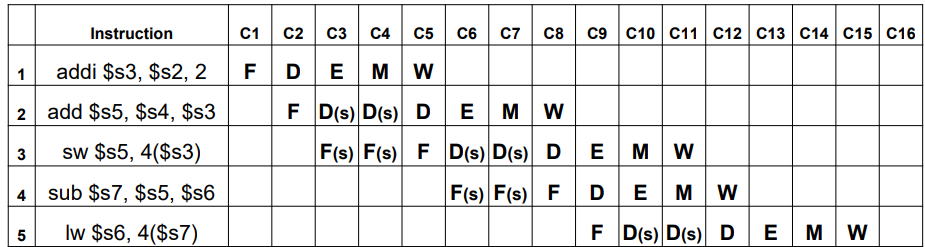
\includegraphics[width=1\linewidth]{images/simp.png}
        \end{figure}
    \item By using forwarding paths we have: 
        \begin{figure}[H]
            \centering
            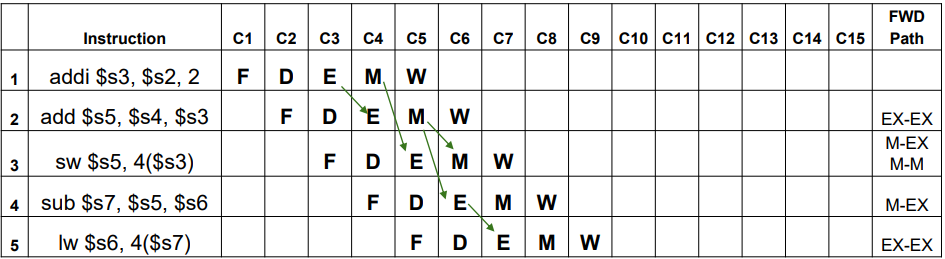
\includegraphics[width=1\linewidth]{images/simp1.png}
        \end{figure}
\end{enumerate}

